\question[20]

\ifspanish

\else

Consider the binary decision problems given by likelihoods
\begin{align*}
p_{X|H}(x|1) &= \frac12 x,    \qquad  0 \le x \le 2,       \\
p_{X|H}(x|0) &= 2(1-x)        \qquad  0 \le x \le 1
\end{align*}

\begin{parts}
\part Compute the decision regions of the LRT with threshold $\eta$
\part Represent, approximately, the ROC of the LRT.
\part Compute the minimax classifier.
\end{parts}

\begin{solution}
\begin{parts}
\part 
For $1\le x \le 2$, $D=1$.

For $0\le x \le 1$, we have
\begin{align*}
p_{X|H}(x|1) &\dunodcero \eta \cdot p_{X|H}(x|0)   \\
	\Leftrightarrow  & \quad \frac12 x     \dunodcero  \eta 2(1 - x)       \\
	\Leftrightarrow  & \quad (1 + 4\eta) x \dunodcero  4 \eta       \\
	\Leftrightarrow  & \quad x \dunodcero \frac{4\eta}{1+4\eta}  = \mu  \\
\end{align*}
\part 
\begin{align*}
\pfa  &= \int_{\mu}^1 2(1-x) dx 
       = \left[-(1-x)^2 \right]_\mu^1 
       = (1 - \mu)^2    \\
\pdet  &= \int_{\mu}^2 \frac12 x dx 
        = \left[\frac{x^2}{4} \right]_\mu^2 
        = 1 - \frac14 \mu^2  
\end{align*}
therefore
\begin{align*}
\pdet = 1- \frac14 (1-\sqrt{\pfa})^2
\end{align*}

\begin{center}
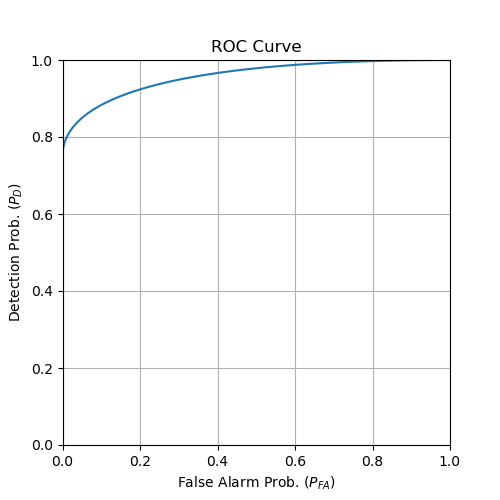
\includegraphics[width=0.4\textwidth]{./Figuras/ROC_202405.png}
\end{center}

\part
\begin{align*}
\pfa = \pmis 
	& \Leftrightarrow \quad (1 - \mu)^2  = \frac14 \mu^2   \\
	& \Leftrightarrow \quad  1 - \mu  = \frac12 \mu    \\
	& \Leftrightarrow \quad  \mu = \frac23
\end{align*}
\end{parts}
\end{solution}

\fi
